
\section{Overview}

\begin{figure}[h!]
\begin{center}
\includegraphics[scale=1.3]{overview.pdf}
\end{center}
\caption{Software Overview}
\label{overview}
\end{figure}

The DSP Assembly is programmed in the ADSP-21262's very verbose assembly language. The software has five principle components.

\begin{itemize}
\item \textbf{Loader:} The boot loader handles the complexity of getting intial code onto the DSP; once a full program has been loaded it transfers execution to that new program. 

\item \textbf{Init:} Post-boot initialization sets up various regions of memory and address register for normal operation, zeros existing buffers, and enables interrupts. 

\item \textbf{Events:} Primary event-processing loop; handles all inbound and outbound events. Decodes them, and sets system state and configuration parameters accordingly. An infinite loop. 

\item \textbf{Timer:} The system timer interrupt subroutine. Every TINC interval, increments the system timestamp counter. 

\item \textbf{Samples:} The primary signal processing interrupt subroutine; the arrival of a new set of samples triggers this interrupt routine, which performs conversion, filtering, spike detection, downsampling, and packetization. 

\end{itemize}

\section{Analog Devices ADSP-21262}

\begin{figure}[h!]
\begin{center}
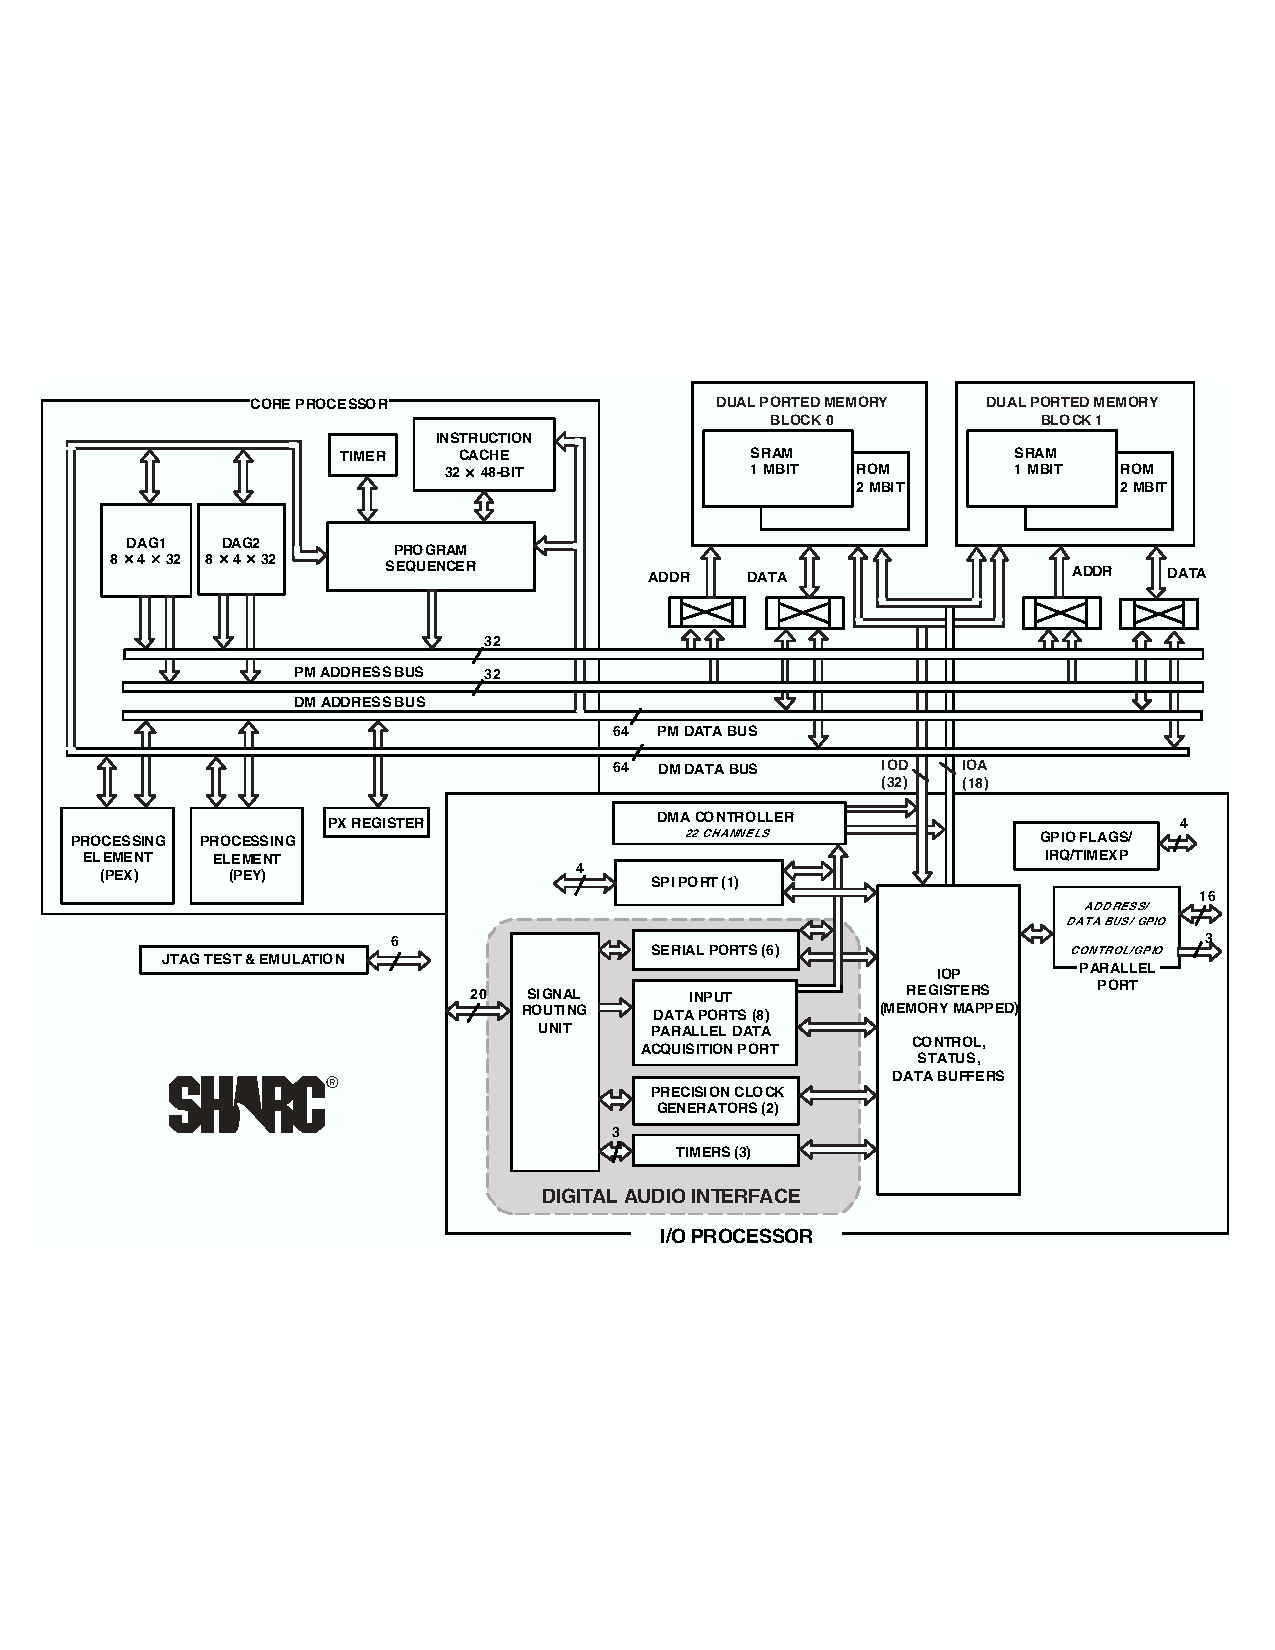
\includegraphics[scale=0.7]{adsp21262.pdf}
\end{center}
\caption{ADSP-21262 Functional Block Diagram. From Analog Devices ADSP-21262 datasheet.}
\label{adsp21262}
\end{figure}

The Analog Devices ADSP-21262 was selected for its extensive on-chip memory, SIMD operation, and inexpensive development tools. The component was available in a PQFP package for easy hand assembly, and can achieve a peak floating point performance of 400 MMACS/sec. 

The DSP contains two blocks of one Mbit of dual-ported SRAM, which in our configuration are used as Program Memory (PM) and Data Memory (DM). Each block has its own 32-bit address bus and 64-bit data bus. 

Something about the dual processing elements

The data address generators:
   1. hardware circular buffering
   2. temporary storage of relevant parameters

Interrupts
   masking
   prioritized

DMA
   overhead
   latency



